%document class
\documentclass{article}


%package
\usepackage{ctex}      % 中文支持
\usepackage{amsmath}   % Advanced math typesetting
\usepackage{amsfonts}
\usepackage{hyperref}  % Add a link to your document
\usepackage{graphicx}  % Add pictures to your document
\usepackage{subcaption}% Add sub figure support
\usepackage{listings}  % Source code formatting and highlighting
\usepackage[backend=bibtex]{biblatex} % Use biblatex package
%\bibliography{cite}	    % Cite database name


%document body
\begin{document}

%============================================
\title{Stanford CS230 Notes}
\author{}
\date{}
\maketitle{}          % Generate title


%contents 目录
\renewcommand{\contentsname}{\centering Contents}
\tableofcontents{}    % Generate contents


\section{Introduction to Deep Learning}


%============================================
\subsection{What is a Neural Network?}
neuron, links.


%============================================
\subsection{Supervised Learning with Neural Networks}
Supervised Learning

Examples:Standard NN, Convolutional NN, Recurrent NN

Structured Data:tabular data; Unstructured Data:audio/image/text


%============================================
\subsection{Why is Deep Learning taking off?}
Amount of labeled data.
\newpage{}
\section{Basics of Neural Network Programming}


%============================================
\subsection{Binary Classification}
\subsubsection{Binary Classification}
image $\rightarrow$ 1 (cat) vs 0 (non cat)

\subsubsection{Notation}
%\begin{align}
	$m$: number of examples

	$n_x$: input size

	$n_y$: output size

	$x$: input, column vector

	$y$: output, 0/1

	$X$: input matrix, shape = $(n_x, m)$

	$Y$: output matrix, shape = $(1, m)$

	$x^{(i)}$: superscript (i) will denote the $i^{th}$ example.
%\end{align}


%============================================
\subsection{Logistic Regression}
Given:
	$x \in \mathbb{R}^{n_x}$, $0 \le \hat{y} \le 1$

Parameters: 
	$w \in \mathbb{R}^{n_x}$, $b \in \mathbb{R}$

Output: 
\begin{align}
	z = w^Tx + b   \\
	\hat{y} = \sigma{(z)} \\
	\sigma{(z)} \approx \frac{1}{1 + e^{-z}} \\
	z \approx \infty, \sigma{(z)} \approx \frac{1}{1 + 0} = 1 \\
	z \approx -\infty, \sigma{(z)} \approx \frac{1}{1 + \infty} = 0
\end{align}

Simplified Parameters:
	$x_0 = 1$, $x \in \mathbb{R}^{{n_x} + 1}$

\begin{align}
	\theta_0 = b, \theta_1 ... \theta_{n_x} = w \\
	\theta = \begin{bmatrix} 
				\theta_0 \\
				\theta_1 \\
				\theta_2 \\
				...      \\
				\theta_{n_x} \\
	         \end{bmatrix} \\
	\hat{y} = \sigma{(\theta^Tx)}
\end{align}


%============================================
\subsection{Logistic Regression cost function}

Given $\{ (x^{(1)}, y^{(1)}, ..., (x^{(m)}, y^{(m)} \}$,
want $\hat{y}^{(i)} \approx {y}^{(i)}$.

Loss (error) function (mean square error/cross entropy):
\begin{align}
	\mathcal{L}(\hat{y}, y) = \frac{1}{2}(\hat{y} - y)^2  \\
	\mathcal{L}(\hat{y}, y) = -(y\log{\hat{y}} + (1-y)\log(1 - \hat{y}))
\end{align}

If y = 1: $\mathcal{L}(\hat{y}, y) = -\log{\hat{y}}$, 
want $\mathcal{L}$ small, want $\hat{y}$ large, want $\hat{y}$ equal to 1.  
If y = 0: $\mathcal{L}(\hat{y}, y) = -\log{(1 - \hat{y})}$,
want $\mathcal{L}$ small, want $\hat{y}$ small, want  $\hat{y}$ equal to 0. 


Cost function:
\begin{align}
	J(w, b) = \frac{1}{m} \displaystyle\sum_{i=1}^m \mathcal{L}(\hat{y}, y) \\
	J(w, b) = - \frac{1}{m} \displaystyle\sum_{i=1}^m [y^{(i)}\log{\hat{y}^{(i)}} + (1 - y^{(i)})\log{1 - \hat{y}^{(i)}}]
\end{align}

Given a random variable $X$ with probability mass function $p_X(x)$, 
the self information of measuring $X$ as outcome $x$ is defined as:
\begin{align}
	I_X(x) = \log[p_X(x)] = \log(\frac{1}{p_X(x)})
\end{align}

Shannon Entroy of $X$:
\begin{align}
	H(X) = \sum_{x} -p_X(x)\log{p_X(x)} \\
	= \sum_{x} p_X(x)I_X(x) \\
	= E[I_X(x)]
\end{align}

Cross Entropy of the the true distributions $p$ and estimated distribution $q$:
\begin{align}
	H(p, q) = E_p[-\log{q}] = -\sum_{x \in \mathcal X} p(x) \log{q(x)}
\end{align}
\newpage{}
\section{Deep Reinforcement Learning}


%============================================
\subsection{Motivation}
\subsubsection{Why RL}
Making sequences of decisions.

Delayed labels. After you take the action, you will know the result.


\subsubsection{What is RL}
Automatically learn to make good sequences of decision.


\subsubsection{Examples}
Robotics

Games

Advertisement


%============================================
\subsection{Recycling Game}
\subsubsection{Q learning}
\begin{figure}[h!] % Here
	\centering
	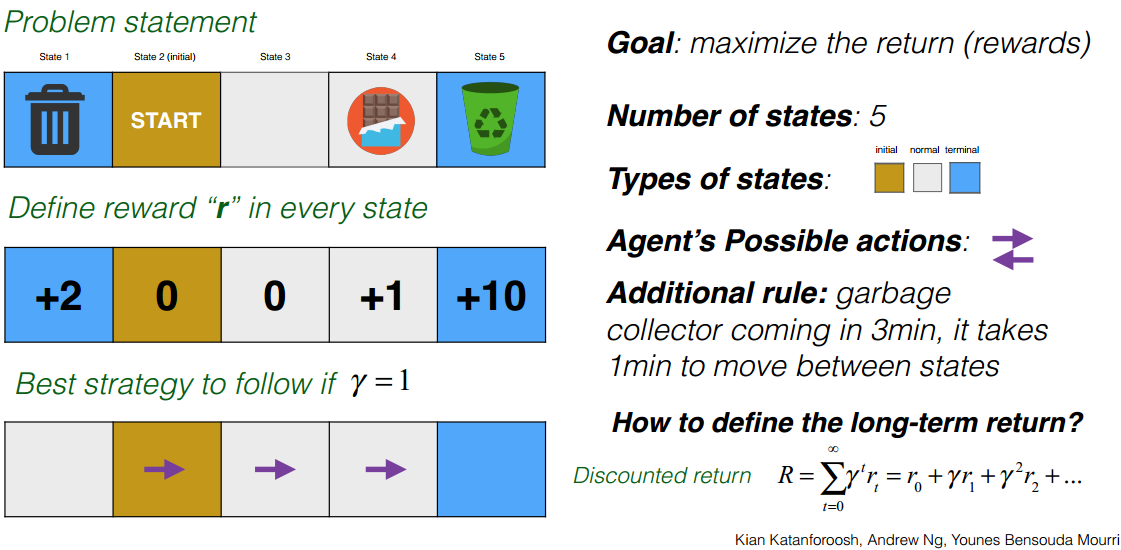
\includegraphics[width=1.0\linewidth]{img/recycling_game_0.png}
	\caption{Game}\label{img:recycling_game_0}
\end{figure}

\begin{figure}[h!] % Here
	\centering
	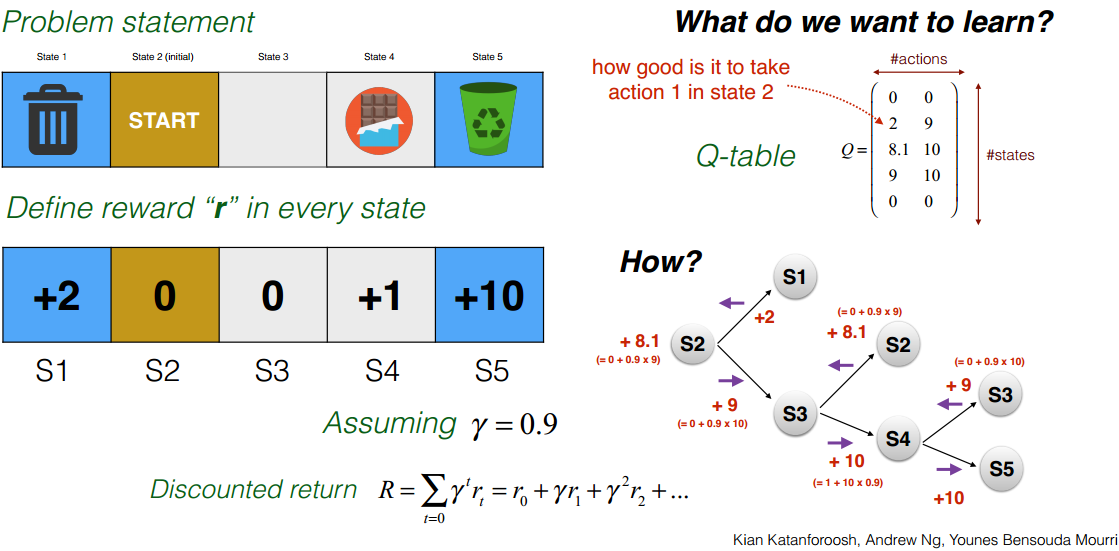
\includegraphics[width=1.0\linewidth]{img/recycling_game_1.png}
	\caption{Q-table}\label{img:recycling_game_1}
\end{figure}

\begin{figure}[h!] % Here
	\centering
	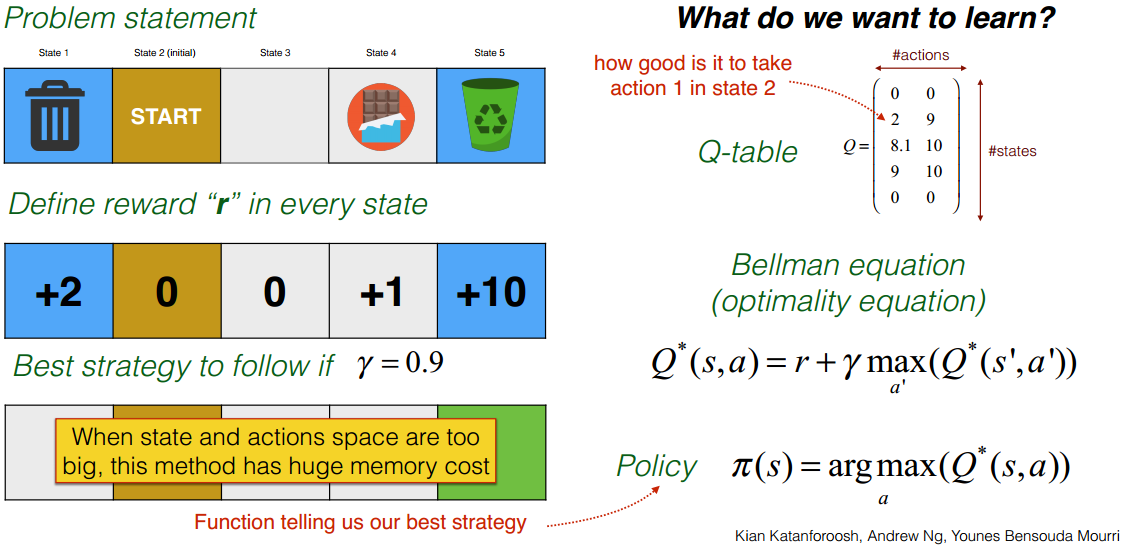
\includegraphics[width=1.0\linewidth]{img/recycling_game_2.png}
	\caption{Bellman equation and Policy}\label{img:recycling_game_1}
\end{figure}

\subsubsection{Summary}
Vocabulary: environment, agent, state, action, reward, total return, 
discount factor/discount rate.

Q-table: matrix of entries representing ``how good is it to take action a
in state s''

Policy: function telling us what's the best strategy to adopt

Bellman equation satisfied by the optimal Q-table


%============================================
\subsection{Deep Q-Networks}

\subsubsection{Main idea}
Main idea: find a Q-function to replace the Q-table

Q-function: Neural Network.

\subsubsection{Deep Q Learning}
\begin{align}
	\hat{y} &= Q(s, a) \\
	L &= (y - \hat{y})^2 \\
	y &= r + \gamma \displaystyle\max_{a'}(Q(s^{next}_a, a')) % // after taking a
\end{align}

Backpropagation:
Compute $\frac{\partial L}{\partial W}$ and update W using stochastic gradient descent.


%============================================
\subsection{Application of Deep Q-Network: Breakout (Ataria)}
\begin{itemize}
	\item Deep Q-network architecture: CNN for image input.
	\item Exploration vs. Exploitation
	\item Implementation:
	\begin{itemize}
		\item Preprocessing
		\item Detect terminal State
		\item Experience replay
		\item Epsilon greedy action
	\end{itemize}
\end{itemize}


%============================================
\subsection{Advanced topics}
Policy Gradient Methods: 
PPO(Proximal Policy Optimization), 
TRPO(Trust Region Policy Optimization).


%bibliography
\newpage{}
\printbibliography

%============================================
\end{document}